\subsection{Encodage positionnel}

La première couche de l'encodeur aussi bien que du décodeur est une couche d'encodage positionnel.
Elle permet de calculer une représentation vectorielle de la séquence en question.
Elle est composée d'une couche de plongement et d'une couche d'encodage de la position.

La couche de plongement mappe chaque élément de la séquence à un vecteur de dimension fixe \(d\),
ainsi transformant une séquence de longueur \(n\) en une matrice de \(\reals^{n \times d}\).
Elle peut avoir une architecture quelconque en fonction de la nature des données.
Il peut s'agir d'une couche de plongement lexical dans le cas d'un texte, 
d'une couche de convolution dans le cas de l'audio 
ou d'une couche récurrente dans le cas d'une série chronologique.

Le transformeur est un invariant aux permutations%
\footnote{%
    Pour une séquence \(x = (x_1, \ldots, x_n)\) et une permutation \(\pi\in S_n\),
    \(x\) et \(\left(x_{\pi(i)}\right)_{1 \le i \le n}\) ont deux encodages identiques.
}.
La sortie de la couche de plongement est donc insuffisante pour représenter la séquence.
Il lui faut ajouter une information sur l'ordre des éléments.
C'est ce que fait la couche d'encodage de la position.
Les auteurs~\cite{attention} proposent l'encodage suivant pour la position \(i\) :
\begin{equation}
    \label{eq.sine-positional-encoding}
    \mathrm{PE}_{k}(i) = 
    \begin{cases}
        \sin\left(\frac{i}{r^{2k/d}}\right) & \text{si } k \text{ est pair} \\
        \cos\left(\frac{i}{r^{2k/d}}\right) & \text{si } k \text{ est impair}
    \end{cases} \qquad 1 \le k \le d
\end{equation}
où \(d\) est la dimension de plongement et \(r\) est un hyperparamètre fixé à \(10^4\) par les auteurs.
La figure~\ref{fig.positional-encoding} montre la matrice d'encodage des \(256\) premières positions
avec \(r=10^4\) et \(d=512\).

\begin{figure}[htb]
    \centering
    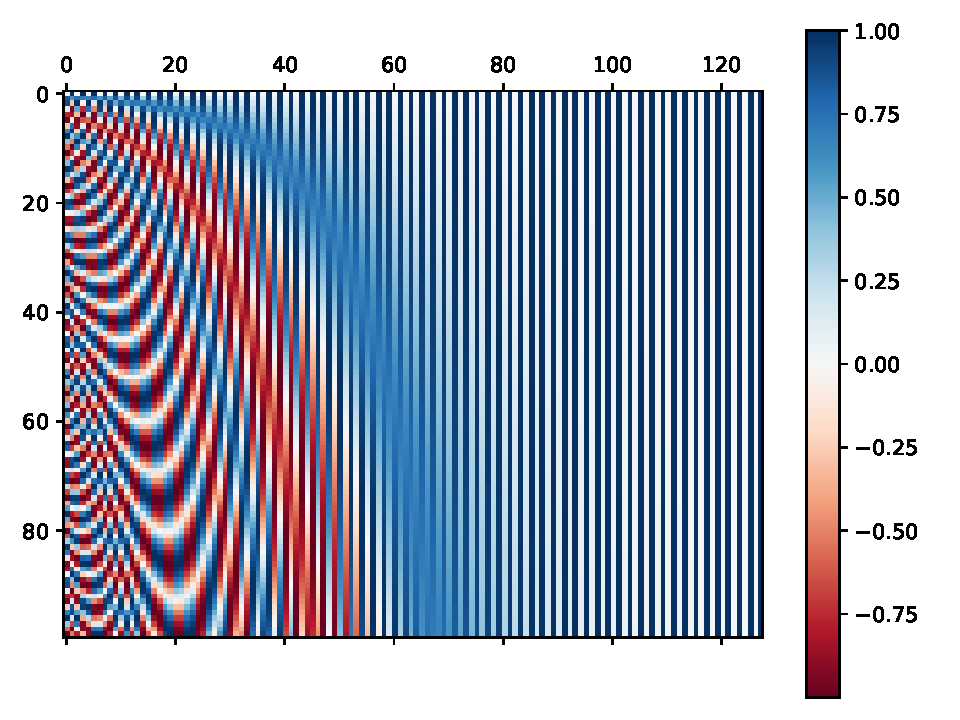
\includegraphics[width=12cm]{assets/python/positional_embedding.pdf}
    \caption{Matrice d'encodage de la position pour \(r=10^4\) et \(d=512\).}
    \label{fig.positional-encoding}
\end{figure}

La représentation finale de la séquence est la somme de la sortie de la couche de plongement 
et celle de la couche d'encodage de la position.
Une couche de plongement lexical peut être substituée à l'encodage donné par
l'équation~\eqref{eq.sine-positional-encoding} avec des résultats similaires~\cite{attention}.

